\section{Evaluation}

\framework is implemented as a C++ library that can be used within a DSL compiler.  It uses the ISL~\cite{verdoolaege_isl:_2010} (Integer Set Library) to represent sets, relations and operations on sets and relations.  To integrate \framework within a DSL compiler the user must generate the following three pieces of information from the DSL IR:
\begin{itemize}
    \item The first layer representation which describes the algorithm;
    \item A set of scheduling commands indicating how the algorithm should be scheduled (commands such as \lstinline{tile()}, \lstinline{split()}, \lstinline{fuse()}, \lstinline{skew()}, \lstinline{parallelize()}, \lstinline{vectorize()}, etc.);
    \item A set of commands declaring the buffers and mapping the computations to buffer elements.
\end{itemize}
The \framework framework will take the three inputs and generate Layer II and Layer III automatically.
%; it will apply the scheduling commands to generate the second layer and then it will add the buffer declaration and add the data mappings to generate layer three.
Then, it will automatically generate an AST (Abstract Syntax Tree) representing the optimized program.  The user can generate the DSL IR back from the AST or can generate any other type of code.  \framework provides an optional code generation path targeting the LLVM IR and another optional code generation path targeting C code.

\subsection{Integrating \framework into the Halide DSL Compiler}

To demonstrate the generality of the proposed framework, we integrated \framework into the Halide compiler~\cite{halide_12}. Halide is a domain specific language and compiler designed for fast image processing.
%It decouples the algorithm, which defines what values are computed, from its schedule, which defines how and when they are computed. This separation of algorithm and schedule allows programmers to explore different scheduling strategies without having to modify the algorithmic code.
To generate the \framework{} IR we proceed as follows: a Halide function (which is equivalent to a statement in a loop nest) is mapped directly to a set of computations in the first layer of \framework.  Reductions, which update the same function, are mapped to \framework computations in a way similar to that described in Section~\ref{layer1}; the iteration domain of the reduction is expanded and a time dimension is added to it.  Halide scheduling directives, such as tiling, splitting, reordering, parallelization, vectorization, etc., are mapped directly to the equivalent high level set of scheduling commands defined in \framework.  Further, \framework supports more scheduling directives currently not supported by Halide, such as loop-fusion and skewing.

\subsection{Evaluation}

We use the following benchmark suite composed of 5 image processing benchmarks:

\begin{description}
\item[Color conversion.] A pixel-wise operation that changes the color representation of each pixel in an image.
 
\item[General 2D convolution.] A two-dimensional convolution of an image implemented by calculating the weighted sum of the area around the pixel using a kernel matrix for weights.  It is used to perform a wide range of image processing operations.

%\item[2D Blur.] A $3\times3$ box filter implemented as separate horizontal and vertical passes.  The first pass computes the average of three pixels on the horizontal axis while the second pass computes the average of three pixels on the vertical axis.

%\item[RGB to YUV420.] An RGB to YUV420 image conversion operation, where the size of the U and V channels are half of the size of the R channel. Due to the difference in the output sizes of the channels, those channels have to be computed in separate loops. This benchmark demonstrates loop fusion by \framework which is not currently supported in the mainstream Halide.  
% Data layout different between CPU and GPU.

\item[Recursive Filter] A simple recursive filter example from RecFilter~\cite{recfilter}, a language built on top of Halide for expressing Infinite Impulse Response (IIR) filters.

\item[Recursive Edge Detector] This is an edge detector that has two stages (two convolutions).  The first convolution reads an input image and creates a new buffer for output.  The second convolution reads the buffer produced by the first convolution and writes in the buffer used as input by the first pipeline (it overrides the input of the first convolution to avoid creating a new buffer for the output).  Implementing this algorithm in Halide is not possible given that it has a recursive definition.

\item[Filter Pipeline] This is an image processing pipeline that takes one input image and computes two separate outputs: the negative of the input image and another brightened copy of the image.% This benchmark demonstrates loop fusion by \framework which is not currently supported in the mainstream Halide.

\end{description}

We performed the evaluation on a dual-socket machine with two 24-core Intel Xeon CPU E5-2680 v3 CPUs running at 2.50GHz running Ubuntu 14.04.5 LTS.

\subsection{Experimental Results}

\begin{figure}
\centering
 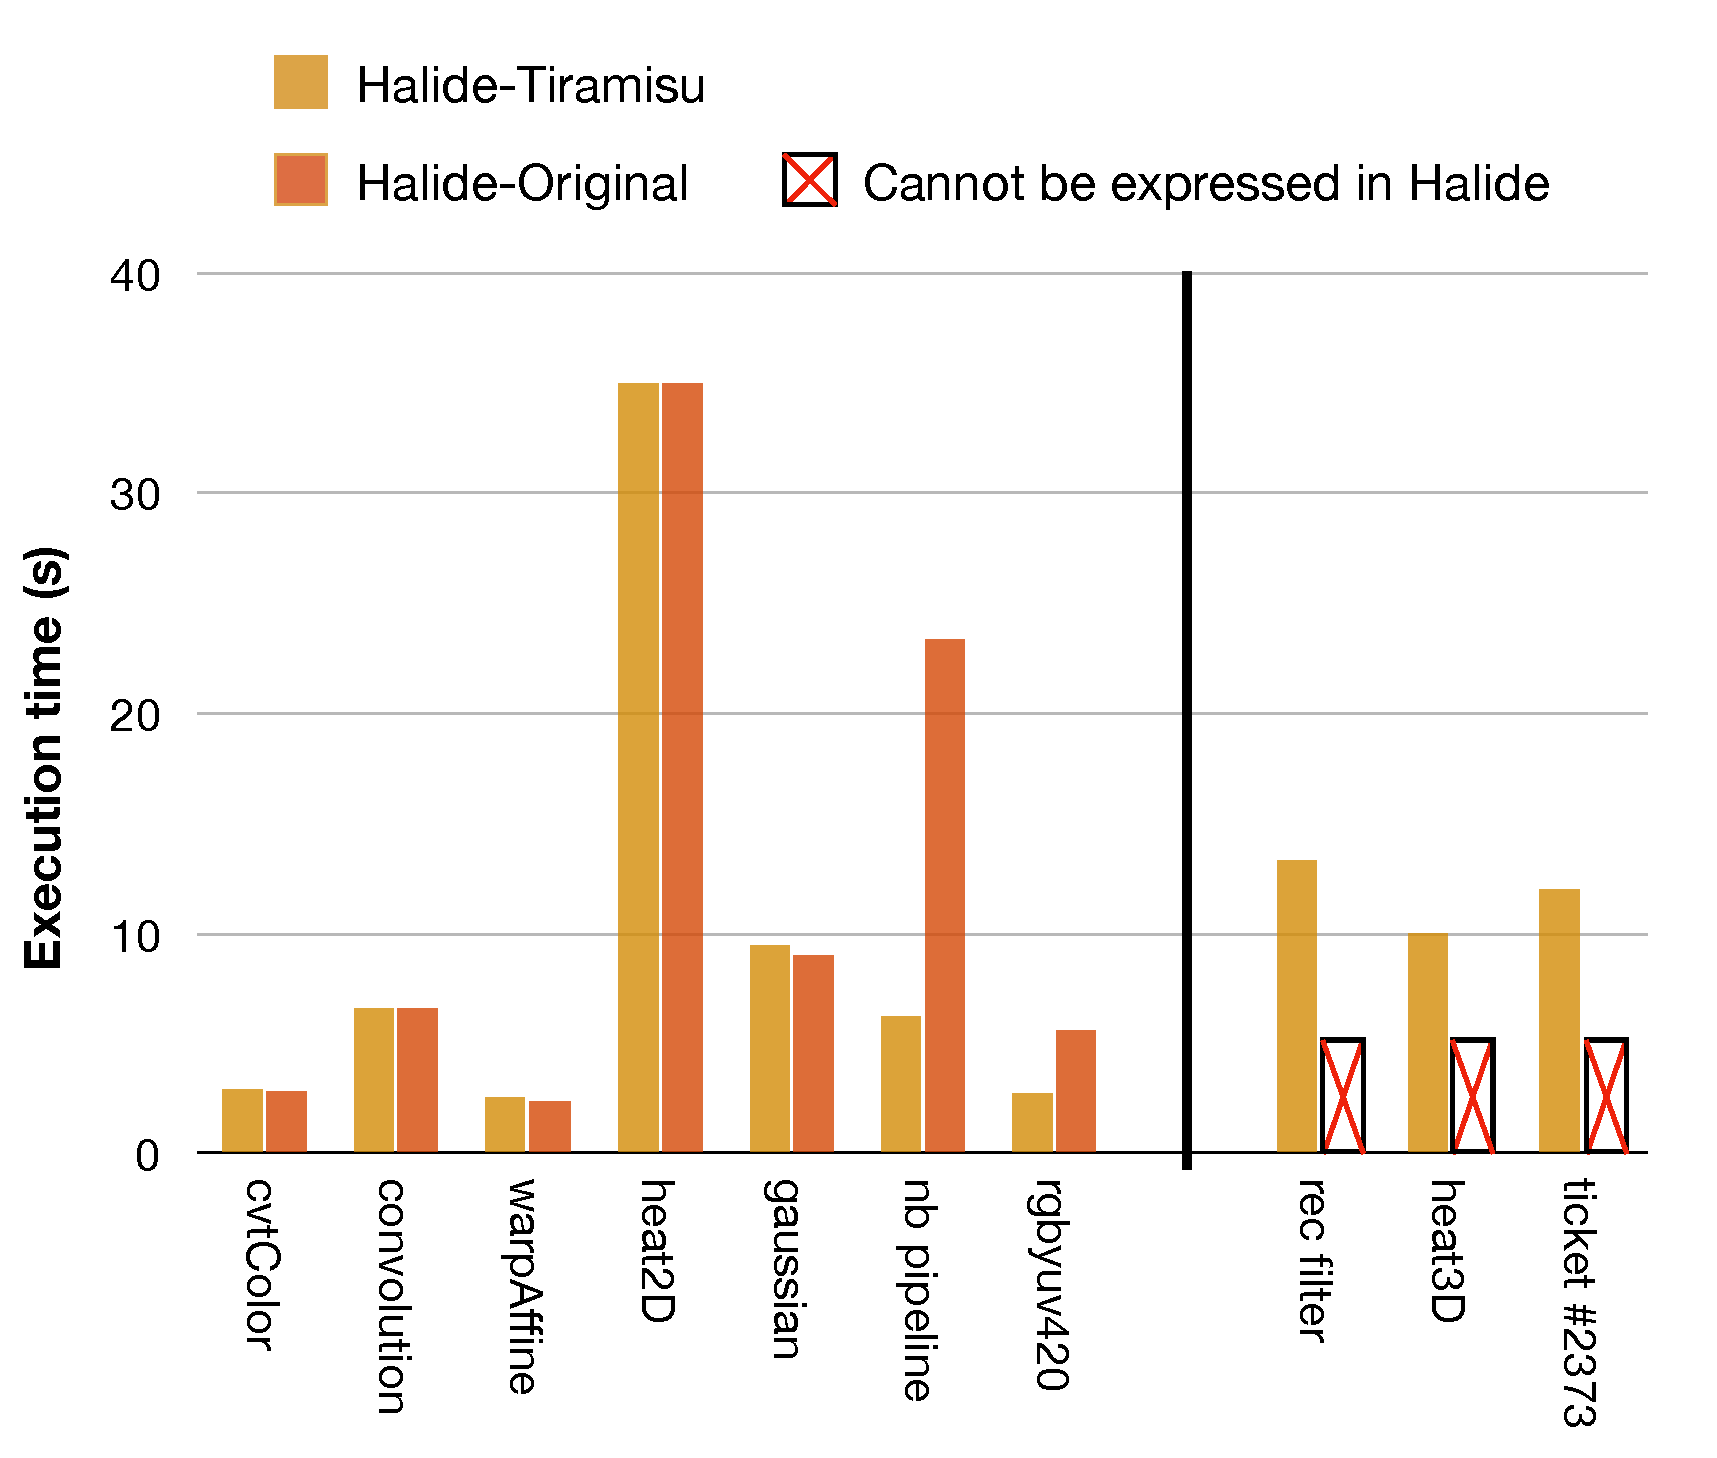
\includegraphics[scale=0.5]{./figures/perf.pdf}
 \caption{Speedup of \framework over Halide}
 \label{fig:speedup}
\end{figure}

We implemented each one of the image processing benchmarks in Halide.  We compile these benchmarks using the original Halide compiler and measure the execution time (we call this compiler Halide-original), then we compile the benchmarks using a modified version of the Halide compiler which uses the \framework framework and measure the execution time (we call this compiler Halide-\framework).  We report the speedup of code generated by the Halide-\framework compiler over the code generated by the Halide-original compiler; the baseline is the Halide-original compiler.

Figure~\ref{fig:speedup} shows the speedups of the \framework framework over Halide.
In three of the benchmarks (\emph{Color conversion}, \emph{2D convolution} and \emph{Recursive Filter}), the performance of the code generated by Halide-\framework matches the performance of the Halide-original.  The same schedule used within Halide-original is generated and used within Halide-\framework.  

The \emph{Recursive Edge Detector} benchmark cannot be implemented in Halide given that it has a recursive definition (Halide does not allow recursive definitions).  Thus we implement the baseline for this benchmark in C rather than Halide.  That C code has two loop nests, the two loop nests can be parallelized but such a parallelism does not provide the best data locality.  In order to get both parallelism and data locality, we need to exploit wavefront parallelism by skewing the iteration space.  Expressing skewing in Halide is challenging since Halide uses an interval based representation in which expressing skewing is not trivial.  The \framework framework uses a polyhedral-based representation that is more expressive than the interval based representation used within Halide and thus \framework can easily express and apply skewing.
When we apply skewing in \framework, the code generated by Halide-\framework is $10.5\times$ faster than the sequential C code and is $2.7\times$ faster than the parallel C code (parallelization without skewing).  This benchmark shows that skewing in this case is good for performance since it enhances both data locality and
parallelism.
The benchmark also provides an example of a complex quasi-affine transformation of the iteration space that is not currently supported by Halide.  This shows the ability of \framework to express complex affine loop nest transformations.

In the last benchmark, \emph{Filter Pipeline}, we have two loop nests that both consume the same image.  Fusing these two loop nests enhances data locality but loop fusion is not currently supported in Halide.  With fusion, we get $3.8\times$ speedup over the non fused Halide code.

\begin{figure}
\centering
 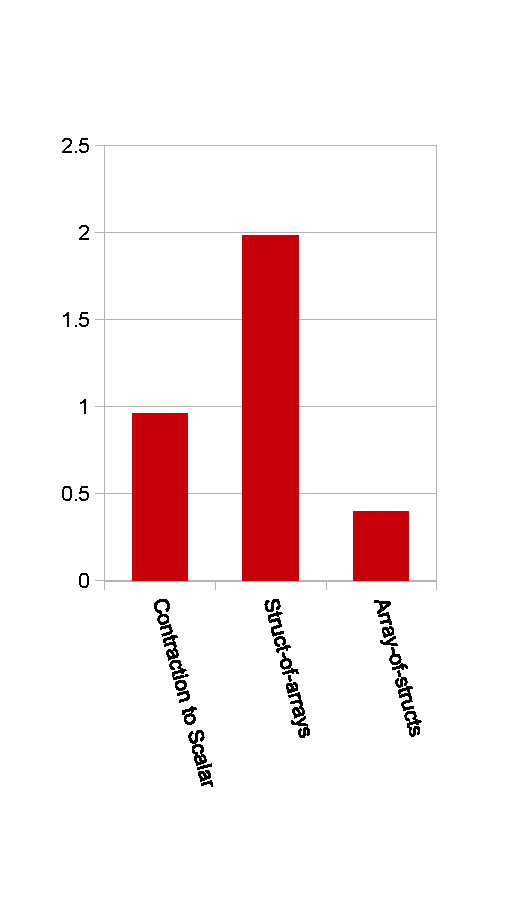
\includegraphics[scale=0.7]{./figures/perf2.pdf}
 \caption{Speedup of \framework over Halide for different data-layouts in an image processing pipeline}
 \label{fig:speedup2}
\end{figure}

Figure~\ref{fig:speedup2} shows the speedup of code generated from Halide-\framework over code generated from Halide-original for different data layouts.  We map the computations of an image processing pipeline to three different data-layouts: full contraction to scalars, struct-of-arrays and array-of-structs.  The goal of this experiment is not to evaluate the gains in performance but rather to show that \framework can actually perform data-layout transformations such as mapping to SOA, AOS and contraction.

\subsection{Integrating \framework into Julia}



\subsection{Integrating \framework into Theano}


\subsection{Tiramisu Code Generators}


Overall, the experiments demonstrated the use of \framework as an IR and an optimization framework for an industrial-strength DSL.  It showed that our implementation matches Halide without losing performance.  In addition, it showed that the three-layer representation allows us to perform advanced loop nest transformations such as skewing which cannot be done in Halide.
The experiments also show that \framework can map computations to different data layouts successfully. % It is up to the user to choose the right data-layout though.
